\documentclass{standalone}
\usepackage{tikz}
\usepackage{ctex,siunitx}
\usepackage{tkz-euclide}
\usepackage{amsmath}
\usetikzlibrary{patterns, calc}
\usetikzlibrary {decorations.pathmorphing, decorations.pathreplacing, decorations.shapes,}
\begin{document}
\small
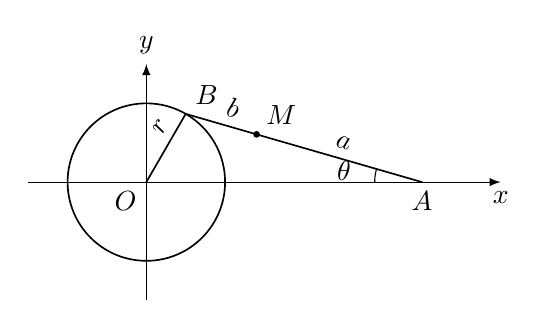
\begin{tikzpicture}[>=latex,scale=1]
  \tkzDefPoints{0/0/O,3.5/0/A}
  \tkzDefPoint(60:1){B}
  \tkzDefPointOnLine[pos=0.7](A,B)\tkzGetPoint{M}
  \draw[thin,->](-1.5,0)--(4.5,0)node[below]{$x$};
  \draw[thin,->](0,-1.5)--(0,1.5)node[above]{$y$};
  \draw [semithick] (0,0)circle(1);
  \tkzDrawSegments[semithick](O,B A,B)
  \tkzDrawPoints[fill=black](M)
  \tkzMarkAngle[size=0.6](M,A,O)
  \tkzLabelAngle[pos=1.0](M,A,O){$\theta$}
  \tkzLabelLine[midway,sloped,above,pos=0.5](A,M){$a$}
  \tkzLabelLine[midway,sloped,above,pos=0.4](M,B){$b$}
  \tkzLabelLine[midway,sloped,above,pos=0.7](O,B){$r$}
  \tkzLabelPoints[above right](B,M)
  \tkzLabelPoints[below left](O)
  \tkzLabelPoints[below](A)
\end{tikzpicture}
\end{document}